% Options for packages loaded elsewhere
\PassOptionsToPackage{unicode}{hyperref}
\PassOptionsToPackage{hyphens}{url}
%
\documentclass[
]{article}
\usepackage{amsmath,amssymb}
\usepackage{lmodern}
\usepackage{iftex}
\usepackage{graphicx}
\ifPDFTeX
  \usepackage[T1]{fontenc}
  \usepackage[utf8]{inputenc}
  \usepackage{textcomp} % provide euro and other symbols
\else % if luatex or xetex
  \usepackage{unicode-math}
  \defaultfontfeatures{Scale=MatchLowercase}
  \defaultfontfeatures[\rmfamily]{Ligatures=TeX,Scale=1}
\fi
% Use upquote if available, for straight quotes in verbatim environments
\IfFileExists{upquote.sty}{\usepackage{upquote}}{}
\IfFileExists{microtype.sty}{% use microtype if available
  \usepackage[]{microtype}
  \UseMicrotypeSet[protrusion]{basicmath} % disable protrusion for tt fonts
}{}
\makeatletter
\@ifundefined{KOMAClassName}{% if non-KOMA class
  \IfFileExists{parskip.sty}{%
    \usepackage{parskip}
  }{% else
    \setlength{\parindent}{0pt}
    \setlength{\parskip}{6pt plus 2pt minus 1pt}}
}{% if KOMA class
  \KOMAoptions{parskip=half}}
\makeatother
\usepackage{xcolor}
\IfFileExists{xurl.sty}{\usepackage{xurl}}{} % add URL line breaks if available
\IfFileExists{bookmark.sty}{\usepackage{bookmark}}{\usepackage{hyperref}}
\hypersetup{
  hidelinks,
  pdfcreator={LaTeX via pandoc}}
\urlstyle{same} % disable monospaced font for URLs
\setlength{\emergencystretch}{3em} % prevent overfull lines
\providecommand{\tightlist}{%
  \setlength{\itemsep}{0pt}\setlength{\parskip}{0pt}}
% \setcounter{secnumdepth}{-\maxdimen} % remove section numbering
\ifLuaTeX
  \usepackage{selnolig}  % disable illegal ligatures
\fi

\title{Corruption is not enough}
\author{Butter}
\date{December 2022}

\begin{document}
\maketitle
\setcounter{tocdepth}{2}
\tableofcontents

\hypertarget{summary}{%
\section{Summary}\label{summary}}

One token, one vote mechanisms are the primary governance mechanisms
used by DAOs. However, one token, one vote and other token voting
governance systems operate as effective plutocracies and are widely
considered vulnerable to
\href{./problems.md\#corruption-problems}{corruption} and
\href{./problems.md\#attack-problems}{attack}.

Large or mature DAOs, and many newer DAOs, have introduced vote
delegation in an attempt to scale governance, mitigate voter apathy, and
alleviate the risks of plutocracy.

However, the most recent and well-known examples of plutocracy are from
DAOs, including ENS DAO, Sushi DAO, and MakerDAO, in which vote
delegation is enabled and sometimes mandatory.

We examine the DAO governance problem space and highlight promising
in-market solutions, including hybrid governance, metagovernance, and
market-based governance.

We propose cryptoeconomics as a viable solution space for further
research and present a prototype that seeks to improve stakeholder
cooperation in DAO Governance through incentives designed to make
corruption an unprofitable strategy.
\hypertarget{motivation}{%
\section{Motivation}\label{motivation}}

\hypertarget{decentralised-autonomous-organisations}{%
\subsection{Decentralised Autonomous
Organisations}\label{decentralised-autonomous-organisations}}

DAOs are a novel form of organisation, uniquely enabled by blockchains.

The components of an organisation include, but are not limited to:

\begin{enumerate}
\def\labelenumi{\arabic{enumi}.}
\tightlist
\item
  an \textbf{objective} or \textbf{purpose}
\item
  a membership policy that produces a set of \textbf{members}
\item
  an~\textbf{allocation mechanism}~(how the organisation allocates
  resources), e.g., capitalism, entrepreneurship
\item
  a~\textbf{governance mechanism}~(how to update the organisation's
  properties), e.g., democracy, board of directors, token-voting
\item
  a~\textbf{standardised store of value} (how to represent the value of
  the organisation's resources), e.g., currency, equity, tokens
\end{enumerate}

Through blockchains, DAOs proffer the benefits of coordinated human
effort at scale without the downsides of centralisation, such as
rent-seeking, corruption, collusion, single-point-of-failure,
bureaucracy, and capture that undermine our existing institutions.

Generally, many DAO proponents expect DAOs to outperform relative to
traditional institutions in the provision of public, common, or club
goods because these are the goods most prone to capture by a centralised
entity, e.g.~the state.

It follows that, if Public Goods DAOs are a successful innovation,
resources will flow from the state to DAOs leading to an increase in the
provision of public goods that do not suffer from the problems caused by
centralisation.

In practice, however, it appears that DAOs may not eradicate these
issues but simply move them through time and
space\href{https://kelsienabben.substack.com/p/towards-a-model-of-resilience-in}{1}.
Hence, our simple DAO implementations remain vulnerable to many of the
issues we expect them to offer an escape from.

\hypertarget{dao-governance}{%
\subsection{DAO Governance}\label{dao-governance}}

\emph{DAO governance involves a network of participants coordinating,
\textbf{without a centralised actor with privileged rights,} to make
decisions in pursuit of some goal or outcome, and is formalised or
defined under set of shared context(s), e.g.~a geography, the law, a
market, a cause, etc.}

DAOs, like other organisations, implement their own endogenous rulesets
that govern all components and the interactions between them, such as
the law in the case of nations, compensation, taxation, resource
allocation, social choice, etc.

DAOs are similarly governed by exogenous policies dictated by their
environment such as the law in the case of corporations, market forces,
international relations, physics, blockchain protocols, etc.

Governance mechanisms are, therefore, the component of DAOs that
mediates all components and the interactions between them. In
particular, the translation of stakeholder preferences into decisions
required for the DAO's instantiation, the enforcement of its boundaries,
and its continued operation in accordance with environmental rules, and
in respect of competing rulesets, i.e.~other DAO governance mechanisms.

A description of a DAO's governance mechanism, including the set of
functions and parameters under the mechanism's control, all components,
and the interactions between them would sufficiently describe the DAO
such that a DAO's governance mechanism could be considered the DAO
itself. Therefore, addressing problems in DAO Governance is potentially
the highest value problem to solve in DAOs today to ensure their
adoption.

\hypertarget{dao-governance-models}{%
\subsection{DAO Governance Models}\label{dao-governance-models}}

\emph{Note: We recognise that token-voting, is democratic in nature but
far from a democracy in the literal sense, however we will use the term
democracy to adhere to convention in the broader literature}

Models include:

\begin{itemize}
\tightlist
\item
  Direct Democracy
\item
  Representative Democracy
\item
  Reputation-based Voting
\end{itemize}

\hypertarget{direct-democracy}{%
\subsubsection{\texorpdfstring{\textbf{Direct
Democracy}}{Direct Democracy}}\label{direct-democracy}}

\textbf{\emph{One token, one vote on every proposal}}

\textbf{Description}

In a direct democracy, token-holders make decisions by voting on
proposals, where each token is equivalent to a vote. Currently, this is
the governance mechanism used by the majority of DAOs, especially
smaller, younger DAOs.

Governance must configure the following parameters:

\begin{itemize}
\tightlist
\item
  Who has the right to create a proposal
\item
  How to convert token votes to a decision, e.g.~majority-rule,
  supermajority, quorum-contingent
\end{itemize}

\textbf{Benefits}

\begin{itemize}
\tightlist
\item
  Bundling financial upside and governance rights aligns risk and
  responsibility which incentivises those with the most to gain from
  price appreciation to make decisions that directly or indirectly
  maximise price appreciation
\item
  This is a copy of the equity system which makes it easy for holders to
  understand
\end{itemize}

\textbf{Limitations}

\begin{itemize}
\tightlist
\item
  Keeps out those who may be affected by governance but don't have the
  capital to acquire governance rights
\item
  Tends towards plutocracy which if left unchecked leads to failure
  through a focus on price appreciation, regardless of negative
  externalities
\end{itemize}

\textbf{Examples}

\begin{itemize}
\tightlist
\item
  PleasrDAO, Aavegotchi, VitaDAO
\end{itemize}

\hypertarget{representative-democracy}{%
\subsubsection{\texorpdfstring{\textbf{Representative
Democracy}}{Representative Democracy}}\label{representative-democracy}}

\textbf{\emph{One token, one vote on every proposal with vote
delegation}}

\textbf{Description}

In a representative democracy, token-holders make decisions by voting on
proposals, where each token is equivalent to a vote, but can also
delegate their voting power to a representative. Delegated voting is
increasingly becoming the most popular governance mechanism, especially
for mature, large DAOs. Governance must configure the following
parameters:

\begin{itemize}
\tightlist
\item
  Who has the right to create a proposal
\item
  How to convert token votes to a decision, e.g.~majority-rule,
  supermajority, quorum-contingent
\item
  Which rights can be delegated and to who
\end{itemize}

\textbf{Benefits}

\begin{itemize}
\tightlist
\item
  Aligns incentives by unbundling financial risk and governance power
  and allocating them to domain experts
\item
  Allows governance rights to accrue to representatives~voters believe
  are best placed to represent their preferences
\item
  Reduces voter apathy
\end{itemize}

\textbf{Limitations}

\begin{itemize}
\tightlist
\item
  As delegation scales, the nuance of voter preferences is diluted to
  the preferences of a smaller subset of voters, i.e.~the delegates,
  which is less representative of the population
\item
  Forces the voter to find a single delegate who represents their entire
  range of preferences across all possible decisions (though tokens
  could be split across wallets or delegation functionality enhanced)
\item
  Allowing voters to delegate enables a more persistent form of voter
  apathy, as seen in our traditional political system
\end{itemize}

\textbf{Examples}

\begin{itemize}
\tightlist
\item
  Uniswap, Gitcoin, Compound, ENS, MakerDAO, AAVE, Radicle, Nouns DAO
\end{itemize}

\hypertarget{reputation-based-voting}{%
\subsubsection{\texorpdfstring{\textbf{Reputation-based
Voting}}{Reputation-based Voting}}\label{reputation-based-voting}}

\textbf{\emph{One person, one vote OR One contribution/reputation unit,
one vote on every proposal}}

\textbf{Description}

Non-transferable voting based on your membership, reputation and, or
contribution.

\textbf{Benefits}

\begin{itemize}
\tightlist
\item
  more equitable
\item
  aligns contribution and power
\item
  not vulnerable to plutocracy
\end{itemize}

\textbf{Limitations}

\begin{itemize}
\tightlist
\item
  only as performant as the system's ability to measure contributions
  and assign relative value
\item
  assumes equal exposure to externalities
\item
  inability to express preference intensity
\end{itemize}

\textbf{Examples}

\begin{itemize}
\tightlist
\item
  Optimism
\end{itemize}
\hypertarget{problems}{%
\section{Problems}\label{problems}}

\hypertarget{problem-space}{%
\subsection{Problem Space}\label{problem-space}}

The problem space is defined as DAO Governance, in particular:

\begin{itemize}
\tightlist
\item
  DAO Governance Attacks
\item
  DAO Governance Corruption
\item
  DAO Governance Capture
\item
  DAO Governance Operations
\end{itemize}

\hypertarget{properties}{%
\subsection{Properties}\label{properties}}

\begin{itemize}
\tightlist
\item
  \textbf{Stakeholder.} Any individual, collective, or entity that
  experiences externalities due to the actions of the DAO,
  e.g.~Token-holder, user, delegate, staker/miner, etc.
\item
  \textbf{Participant.} Any individual, collective, or entity that
  participates in governance
\item
  \textbf{Preference.} A stakeholder's subjective comparative
  evaluations over a range of options, e.g.~a miner prefers to increase
  the block reward, over reducing rewards or keeping rewards constant
\item
  \textbf{Objectives.} The goal or set of goals that constitute the
  DAO's organizing purpose, e.g.~``Buy the constitution'', ``Fund Public
  Goods''
\item
  \textbf{Acts.} The set of actions or decisions the DAO's governance
  mechanism is able to produce and its stakeholders consider, e.g.~Add a
  new asset as collateral in our lending protocol, remove a particular
  voter's voting power, increase token supply, offboard a contributor,
  suspend the protocol
\item
  \textbf{Outcomes.} The set of outcomes the DAO's governance mechanism
  is able to achieve through its actions, e.g.~Token Price increases or
  remains stable, protocol users increase
\end{itemize}

\hypertarget{dimensions}{%
\subsection{Dimensions}\label{dimensions}}

To measure the effectiveness of a DAO's governance, we consider the
following dimensions:

\begin{itemize}
\tightlist
\item
  \textbf{Stakeholder Representation.} The distribution of voting power
  relative to DAO stakeholders, i.e.~users, token holders, stakers,
  liquidity providers, etc.
\item
  \textbf{Preference Representation.} The degree to which governance
  participants are able to express their preferences with respect to the
  DAO's objectives, e.g.~I do not believe the voting mechanism is
  legitimate
\item
  \textbf{Alignment.} The consistency of a decision when compared to a
  desired outcome
\item
  \textbf{Coherence.} The consistency of a series of decisions when
  compared to one another, with respect to a desired outcome
\item
  \textbf{Legitimacy.} Power granted by governance participants to the
  governance mechanism through their ongoing implicit agreement to be
  bound by its decisions
\end{itemize}

\hypertarget{problems-1}{%
\subsection{Problems}\label{problems-1}}

\hypertarget{corruption-problems}{%
\subsubsection{Corruption Problems}\label{corruption-problems}}

\hypertarget{opportunism}{%
\paragraph{Opportunism}\label{opportunism}}

Where a single stakeholder or group of stakeholders is rewarded for
acting in their own self interest while punishing all other stakeholders
and producing outcomes that do not align with the DAO's objectives.

\textbf{Example:} Proposing or voting for salary increases or against
salary cuts during a budget-cutting exercise.

\textbf{Symptoms:} - Deviation between outcomes and objectives -
Increase in actions or decisions that do not align with objectives -
Illegitimate diversion of funds

\hypertarget{capture}{%
\paragraph{Capture}\label{capture}}

Where a minority group of stakeholders possess the power to dictate the
DAO's actions to serve their own preferences while punishing all other
stakeholders and producing outcomes that do not align with the DAO's
objectives.

\textbf{Example:} Plutocracy, Bureaucracy

\textbf{Symptoms:} - Deviation between outcomes and objectives -
Increase in actions or decisions that do not align with objectives -
Illegitimate diversion of funds

\hypertarget{collusion}{%
\paragraph{Collusion}\label{collusion}}

Where two or more stakeholders or stakeholder groups that operate within
or outside the boundaries of the DAO cooperate for their mutual benefit,
to the detriment of all other stakeholders and the DAO's ability to
achieve its objectives.

\textbf{Example:}
\href{https://hackingdistributed.com/2018/07/02/on-chain-vote-buying/}{Vote
Buying}

\textbf{Symptoms:} - Deviation between outcomes and objectives -
Increase in actions or decisions that do not align with objectives -
Illegitimate diversion of funds

\hypertarget{attack-problems}{%
\subsubsection{Attack Problems}\label{attack-problems}}

\hypertarget{capital-structure-exploitation}{%
\paragraph{Capital Structure
Exploitation}\label{capital-structure-exploitation}}

Where an individual or group is able to exploit vulnerabilities in the
DAO's governance mechanism to extract capital.

\textbf{Example:} Treasury Drain Attacks, Price Manipulation Attacks,
Arbitrageurs, etc.

\textbf{Symptom:} - Illegitimate diversion of funds

\hypertarget{operation-problems}{%
\subsubsection{Operation Problems}\label{operation-problems}}

\hypertarget{inertia-or-gridlock}{%
\paragraph{Inertia or gridlock}\label{inertia-or-gridlock}}

Governance is not able to produce decisions that meet the demands of DAO
participants or does not reliably produce decisions that align with the
objectives of the DAO.

\textbf{Example:} Infighting, voter apathy, failure to achieve quorum

\textbf{Symptom:} - Reduction in actions and decisions that align with
objectives
\hypertarget{governance-innovations}{%
\section{Governance Innovations}\label{governance-innovations}}

DAO Governance, unlike corporate and public governance, is both public
and open source. The principles of the open source community,
specifically the ability for anyone to copy and reuse code provides many
opportunities for governance innovation---some of which we've shared
above.

\emph{Metagovernance,} \emph{Hybrid Governance,} and \emph{Market
Governance} are three categories of governance innovation that may offer
effective solutions to governance attacks, corruption, and capture.

\hypertarget{metagovernance}{%
\subsection{Metagovernance}\label{metagovernance}}

Metagovernance, in the context of DAOs, is the term commonly used to
describe any activity where one governance mechanism, typically a DAO,
exerts influence on the governance of another DAO.

Metagovernance is a transparent, often automated, vote buying mechanism
that incentivises a target DAO's token-holders to take an action that
benefits the mechanism's stakeholders, e.g.~influence over governance
decisions, direction of token emissions, etc.

Metagovernance creates a secondary set of incentives, or
meta-incentives, that augment the behaviour of primary token-holders.

In one-off instances of metagovernance, such as in the case of FEI and
Index Coop, the Fei team were able to gain influence in AAVE's
governance using Index Coop's token holdings.

There are also extended forms of metagovernance with DAOs whose entire
purpose is to control the governance of other DAOs, such as Convex
Finance.

\hypertarget{curve-emissions-with-convex-finance}{%
\subsubsection{Curve emissions with Convex
Finance}\label{curve-emissions-with-convex-finance}}

Convex was designed to maximise control over CRV emissions on the Curve
protocol.

Convex works by reimplementing Curve's vote-escrow token mechanics to
pay CRV holders with CVX emissions to lock their CRV tokens in Convex's
contract. Convex, in turn, lock these CRV tokens using Curve's contracts
to receive the maximum CRV emissions, which they share with CVX holders,
and voting power, which they use to vote for greater token emissions on
the token pairs selected by CVX holders.

As of this writing, the Convex protocol controls 51\% of all
vote-escrowed CRV, an indicator of the effectiveness of meta-incentives
in one-token, one-vote governance mechanisms.

\hypertarget{redacted-cartel-hidden-hand}{%
\subsubsection{Redacted Cartel, Hidden
Hand}\label{redacted-cartel-hidden-hand}}

Hidden Hand from Redacted Cartel facilitates vote-buying campaigns for
participating DAOs.

Vote buyers, or bribers, deposit bribes for active proposals from a
number of partner DAOs and users delegate governance tokens to Hidden
Hand's protocol. The protocol then distributes votes to maximise returns
for its users in exchange for a 4\% commission of the bribes received.

As an example, \$851,364~worth of bribes were deposited for~61~proposals
on Aura Finance and \$2,346,024 was deposited for~27~proposals on
Balancer.

Hidden Hand also allows partners to implement their own bribe
marketplaces so users can select which bribes to accept in exchange for
their votes.

\hypertarget{fei-asset-listing-on-aave-with-index-coop}{%
\subsubsection{FEI Asset Listing on AAVE with Index
Coop}\label{fei-asset-listing-on-aave-with-index-coop}}

Index Coop, a provider of token indexes, actively encouraged
metagovernance for a small number of the tokens held in their DeFi Pulse
Index, namely Maker, AAVE, and Compound, which they named
metagovernance-as-a-service.

Under this arrangement, holders of INDEX tokens acquired the ability to
use governance tokens held to facilitate DPI's role as an index to make
proposals or vote on proposals within MakerDAO, Aave, and Compound.

In September 2021, FEI protocol, a stablecoin issuer, created a proposal
to list the FEI token on AAVE, using the AAVE token holdings in Index
Coop's DPI.

AAVE's governance, specifically, requires 80,000 AAVE tokens before a
holder can make a governance proposal. At that time, AAVE was trading at
\$327.04, setting the price of making proposals on AAVE at over \$26m.

FEI were able to use \$4m of INDEX tokens to control over 118,000 AAVE,
worth \textasciitilde\$36m allowing the team to successfully list their
token on AAVE.

\hypertarget{hybrid-governance}{%
\subsection{Hybrid Governance}\label{hybrid-governance}}

Hybrid governance is here defined as the combination of two or more
governance models within a single DAO governance mechanism.

This approach is typically pursued where DAO governance designers
believe that outcomes can be better-aligned to the DAO's objectives by
limiting the influence of a group of stakeholders who may be
over-represented in a one-token, one-vote model. Alternatively, hybrid
governance could be implemented to give greater weight to the
preferences of group of stakeholders who are underrepresented or have no
means to express their preferences except to ``vote with their feet'',
which is a loss for all stakeholders.

Hybrid governance modulates the influence of one set of stakeholders by
distributing voting rights to another set of stakeholders, especially
groups whose may be marginalised by the preferences of the dominant
voting bloc.

Voting power is redistributed until each group is able to provide
sufficient checks and balance on the power of other groups.

\hypertarget{lidos-steth-dual-governance}{%
\subsubsection{Lido's stETH Dual
Governance}\label{lidos-steth-dual-governance}}

LidoDAO's is governed by LDO holders. Unfortunately, users that stake
ETH in the Lido contract receive stETH, which confers the holder no
voting rights.

This structure allows Lido holders to make decisions that benefit LDO
holders at the expense of stETH holders.

The goal of Lido's Dual Governance proposal ``is to prevent the Lido DAO
governance from changing the covenant between the protocol and stakers
without consent from the latter.''

The proposal grants stETH holders a vetocracy over proposals that are
deemed to break the agreement under which users stake their ETH on Lido.
stETH holders can signal their disagreement with a proposal by staking
stETH in a vote escrow contract and once a minimum threshold is reached
the proposal will be temporarily blocked to allow the community to
negotiate. stETH holders can vote to block, amend, or pass the proposal
after negotiations.

This power gives stETH enough power to limit opportunism on behalf of
LDO token holders without burdening stakers with ongoing governance
overheads.

\hypertarget{optimisms-hybrid-governance}{%
\subsubsection{Optimism's Hybrid
Governance}\label{optimisms-hybrid-governance}}

Optimism, through the optimism collective have implemented a bicameral
legislative process, comprising a `Token House' within which voting
powers are granted through token ownership, and a `Citizens' House',
within which voting powers are granted through non-transferrable NFTs or
``soulbound tokens''.

The team explains that this approach is ``a large-scale experiment
in~\href{https://vitalik.ca/general/2021/08/16/voting3.html}{non-plutocratic
governance}'' but, so far, there are limited details though the
Citizen's House's remit appears to be reserved for retroactive public
goods funding whereas the Token House has a more traditional DAO
governance remit, e.g.~governance fund~grants, protocol upgrades,
director removal, etc.

\hypertarget{market-governance}{%
\subsection{Market Governance}\label{market-governance}}

Market Governance is co-opted from
\href{https://en.wikipedia.org/wiki/Market_governance_mechanism}{Market
Governance Mechanisms} to describe a mechanism that leverages the
competitive forces of the open market to influence the behaviour of
stakeholders.

As DAOs have scaled in scope, market cap, and contributors, governance
has run into issues of corruption, inertia, and in-fighting, especially
where the DAO's operations are complex.

As the range and diversity of stakeholders increases, and the potential
set of actions and decisions expand, governance must increase its
throughput to accommodate, without creating a self-serving bureaucracy.

\hypertarget{makerdaos-metadaos}{%
\subsubsection{MakerDAO's MetaDAOs}\label{makerdaos-metadaos}}

The solution proposed by Rune in Endgame is a decomposition of Maker
into a single core DAO comprising the main functions of the Maker
protocol and a collection of smaller ``MetaDAO'' governance units with
their own governance and governance token with the freedom to pursue any
viable market opportunity while leveraging some of the resources of the
core DAO.

This innovation affords MakerDAO the ability to maintain a small set
number of governance-controlled parameters for the core protocol, while
the market provides the incentives to steer governance for its MetaDAOs.

This governance upgrade is in the process of being deployed at MakerDAO
so its efficacy is yet to be measured.
\hypertarget{proposal}{%
\section{Proposal}\label{proposal}}

Each governance innovation provides a solution to an aspect of DAO
Governance.

\emph{Metagovernance} provides a system of secondary incentives to
reward or punish governance participants for taking a set of desirable
actions.

\emph{Hybrid Governance} redistributes voting power among stakeholders
using secondary governance mechanisms to create a system of checks and
balances on those who accrue majority power in the primary mechanism.

\emph{Market Governance} decomposes governance into self-contained
organisations and leverages market forces to create alignment between
each group as a limit on bureaucracy and corruption.

These mechanisms improve stakeholder cooperation and alignment using a
system of incentives that originate from three sources.
\emph{Metagovernance} incentives are provided by a mechanism or
protocol. \emph{Hybrid Governance} creates a system of punishments for
corruption, which are provided by other stakeholders or peers.
\emph{Market Governance} incentives are provided by the market through
competition.

Should governance attack, corruption, or capture be detectable by a
governance mechanism, other stakeholders, or competing mechanisms, a set
of economic incentives can be designed to offset the proceeds of these
acts, rendering them unprofitable.

Through our investigations in the field of cryptoeconomics, we aim to
design a mechanism or collection of mechanisms capable of providing
sufficient guarantees about cooperative behaviour in DAOs.

Next, we present an initial exploration in this direction.
\hypertarget{molten}{%
\section{Molten}\label{molten}}

\emph{Molten is WIP. This document will be updated as we conduct ongoing
research and development}

Molten offers permissionless deployment of hybrid governance mechanisms
in a DAO.

\hypertarget{actors}{%
\subsection{Actors}\label{actors}}

Molten is designed to coordinate the actions of three actors:

\textbf{Fundraisers.} Stakeholder with the objective to accrue voting
power to express their preferences, but lack resources. Equivalent to a
delegate in a DAO with vote delegation.

\textbf{Liquidity Providers.} Stakeholder with the objective to accrue
voting power to express their preferences, and have adequate resources.

\textbf{DAO Governance.} Governance mechanism with the objective to
secure and allocate resources in pursuit of its objective.

\hypertarget{components}{%
\subsection{Components}\label{components}}

Molten is comprised of:

\textbf{Fundraiser Contract.} Contract created by Fundraisers to store
liquidity, lock Governance Tokens, and issue mTokens. Contract also
exposes \texttt{exchange} function which can be called by the target
DAO's treasury address.

\textbf{mTokens.} Tokens issued to Liquidity Providers following a
successful exchange. Each token represents a claim on the underlying
governance tokens locked in the Fundraiser contract.

\textbf{Price Oracle} Oracle used to determine the governance token
exchange rate when the \texttt{exchange} function is called.

\hypertarget{operation}{%
\subsection{Operation}\label{operation}}

Molten functions by:

\begin{enumerate}
\def\labelenumi{\arabic{enumi}.}
\item
  Pooling liquidity from minority stakeholders for DAO governance
  tokens, thereby incentivizing DAOs to sell governance tokens and
  distribute voting power in exchange for deep on-chain liquidity
\item
  Locking governance tokens in a contract under the control of its
  owner, the fundraising stakeholder responsible for deploying the
  contract, or another governance mechanism, incentivizing stakeholders
  to seek governance corruption or capture where there are opportunities
  to aggregate and represent minority interests in exchange for voting
  power
\item
  Issuing governance token derivatives to liquidity providers,
  redeemable at maturity for the underlying governance tokens and free
  to trade on secondary markets, while amplifying their preferences
  through vote delegation, incentivizing liquidity providers to seek out
  stakeholders that suitably represent their preferences
\item
  Granting governance token derivative holders a means to liquidate the
  contract, for a penalty, if the fundraising stakeholder is no longer
  voting in-line with their preferences, incentivizing fundraising
  stakeholders to avoid deviating from their agreement with liquidity
  providers when voting in the target DAO
\end{enumerate}

\hypertarget{outcome}{%
\subsection{Outcome}\label{outcome}}

Molten combines both peer incentives, used to incentivize participants
to identify governance capture and corruption and increase stakeholder
cooperation, and market incentives, to surface and distribute voting
power to the most competent and motivated stakeholders capable of
keeping powerful voters in check.

We expect peer incentives will provide sufficient rewards to
stakeholders that identify corruption or
capture\href{https://doi.org/10.1371/journal.pcbi.1004232}{2}, in the
form of delegated voting power, to limit potential gains from either
strategy. We expect market incentives to provide sufficient incentives
to encourage cooperation across stakeholders and inform DAO Governance
through the proportion of tokens locked in a given mechanism.

\hypertarget{implementation}{%
\subsection{Implementation}\label{implementation}}

A prototype implementation can be seen \href{}{here}.

\appendix
\hypertarget{molten-v1}{%
\section{Molten v1}\label{molten-v1}}

\begin{figure}
\centering
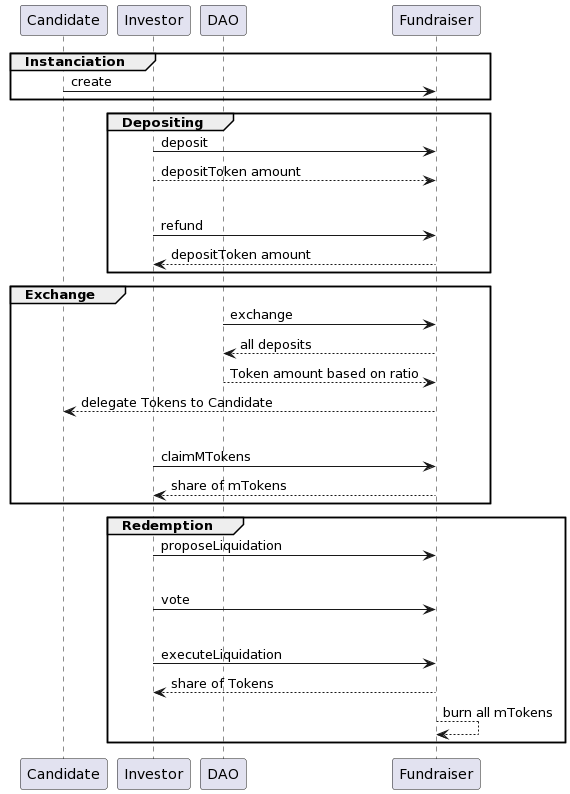
\includegraphics[width=\textwidth]{./img/molten-fundraiser-v1-seq-diag.png}
\caption{Sequence diagram}
\end{figure}

\end{document}
